\documentclass{article}
\usepackage[utf8]{inputenc}
\usepackage{geometry}
\usepackage{graphicx}
\usepackage{hyperref}

\geometry{ left=25mm, right=25mm, top=20mm, bottom=20mm }

\title{\textbf{Report N°2 MSc Thesis: Active Constraints}}
\author{\textbf{Alberto Rota} - \textit{Supervisor: Prof. Elena De Momi}}
\date{}

\begin{document}
\maketitle
\paragraph{Title:} \textit{To Be Defined}
\section*{General guidelines}
    Development of surgical training tasks implementing Active Constraints of
    different nature and with different levels of intervention, in order to
    evaluate their efficacy and role in Robot-Assisted Minimally Invasive
    Sugery.
    \begin{itemize}
        \item \textit{Phase 1: }Software Development in a virtual environment
        (Unity)
        \item \textit{Phase 2: }Implementing on the dVRK, followed by
        experimental tests with data gathering, analysis and validation
    \end{itemize}

\section*{Work planned from the previous Report}

\begin{itemize}
    \item
    Using "Active Constraints/Virtual Fixtures: A survey" as a guide,    
    implementing at least one of every kind of virtual fixture described in the
    paper and in the cited and referenced literature (guidance / avoidance /
    redirection, trajectory / surface / volume-based / force-field,
    static/dynamic, \textit{etc.}).
    \item 
    Literature research and first implementation (software-wise) of real
    surgical tasks (not limited to surgical training) where to apply the virtual
    fixtures implemented above. 
\end{itemize}
\section*{Progress}
    \begin{itemize}
        \item Implemented the \textit{Surface Guidance Active Constraint}
        described in "Dynamic 3-D Virtual Fixtures for Minimally Invasive
        Beating Heart Procedures"
        \href{https://ieeexplore.ieee.org/document/4579344}{(link here)}, which
        functions properly in the virtual surgical scenario
        \item Implemented  the \textit{Guidance-on-insertion Active Constraint}
        described in "Vision-assisted control for manipulation using virtual
        fixtures" \href{https://ieeexplore.ieee.org/document/1362691}{(link
        here)}
        \item Implemented  the \textit{Force-field-based Obstacle Avoidance 
         Active Constraint}
         described in "Real-Time Obstacle Avoidance for Manipulators and Mobile
         Robots"
        \href{https://ieeexplore.ieee.org/document/1087247}{(link
        here)}
        \item Built a way of evaluating the surgeon performance while performing
        the task. The planned trajectory, the executed trajectory and the force
        generated from the active constraint can be exported and read, visualized
        and analyzed through a simple MATLAB script (for now, planning to move
        to Python)
        \item Identified in "Objective evaluation of expert and novice performance
        during robotic surgical training tasks"
        \href{https://link.springer.com/article/10.1007/s00464-008-9933-9}{(link
        here)} and in its cited literature a guide for choosing, constructing
        and evaluating surgical training tasks 
        \item Studied the concepts necessary for building a virtual surgical
        simulation in Unity (collision detection, object pick\&place, \textit{etc.})
    \end{itemize}
\section*{Next Steps}
    \begin{itemize}
        \item Implementing the last few remaining virtual fixtures described
        in "Active Constraints/Virtual Fixtures: A survey" and in the related literature
        \item Creating at least one functional surgical task in the virtual
        environment in Unity
    \end{itemize}
\newpage
\section*{Screenshots}
\begin{figure}[h!] \begin{small} \begin{center}
    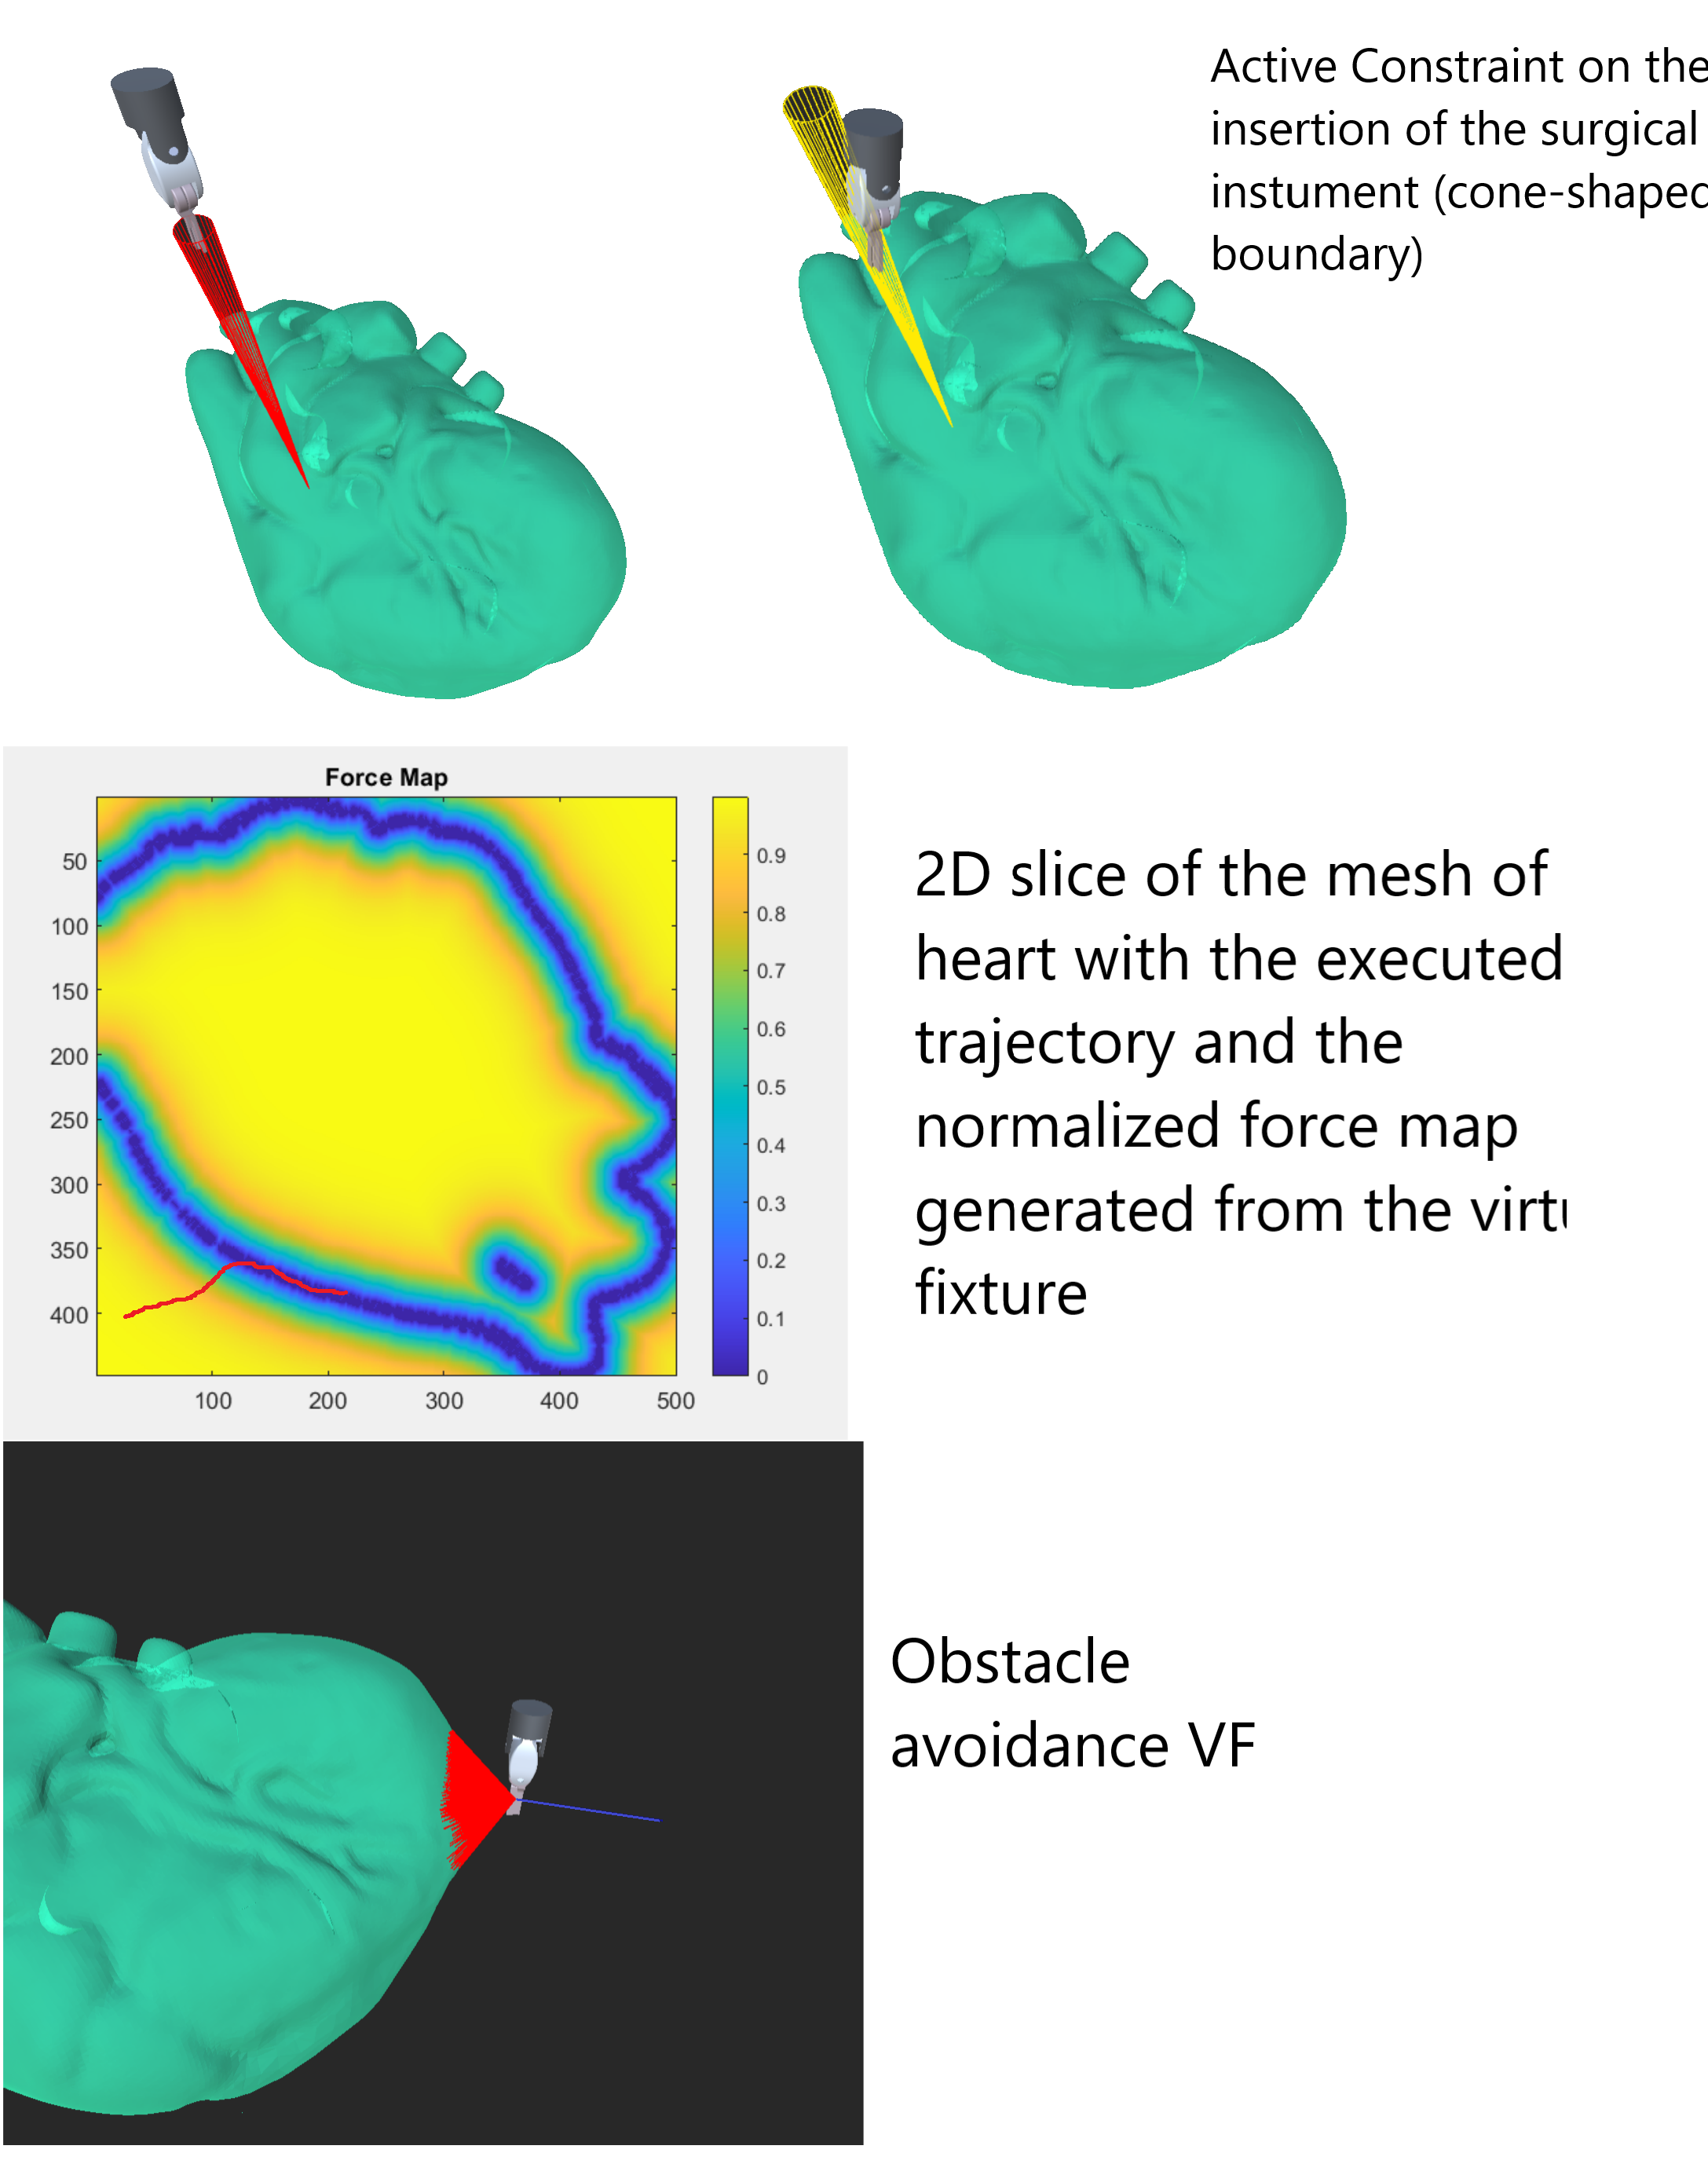
\includegraphics[width=0.95\textwidth]{Scene.png} \end{center}
    \label{fig:} \end{small} \end{figure}
\end{document}